\section{Methods for prediction and analysis of roll damping}
\label{se:methods_for_prediction_and_analysis}

\subsection{Hydrodynamics}
\label{se:hydrodynamics}
The roll damping consists of linear and nonlinear components. At zero speed the nonlinear damping is caused by the two-dimensional separation at the bilge keel or near the bilge circle (Eddy damping $B_E$). While at speed the nonlinear damping is mainly caused by the hydrodynamic lift force on the hull, represented as lift damping $B_L$. $B_E$ vanishes at high speed ($F_n>0.15)$ \cite{ikeda_components_1978}.

The wave damping also changes at speed. Ikeda \cite{ikeda_components_1978} proposes a formula for the fraction between wave damping at speed and zero speed: $\frac{B_W}{B_{W0}}$

The Ikeda method has been used to calculate the roll damping for a PCTC vessel Faust \cite{soder_assessment_2019}.
\begin{figure}[h]
    \centering
    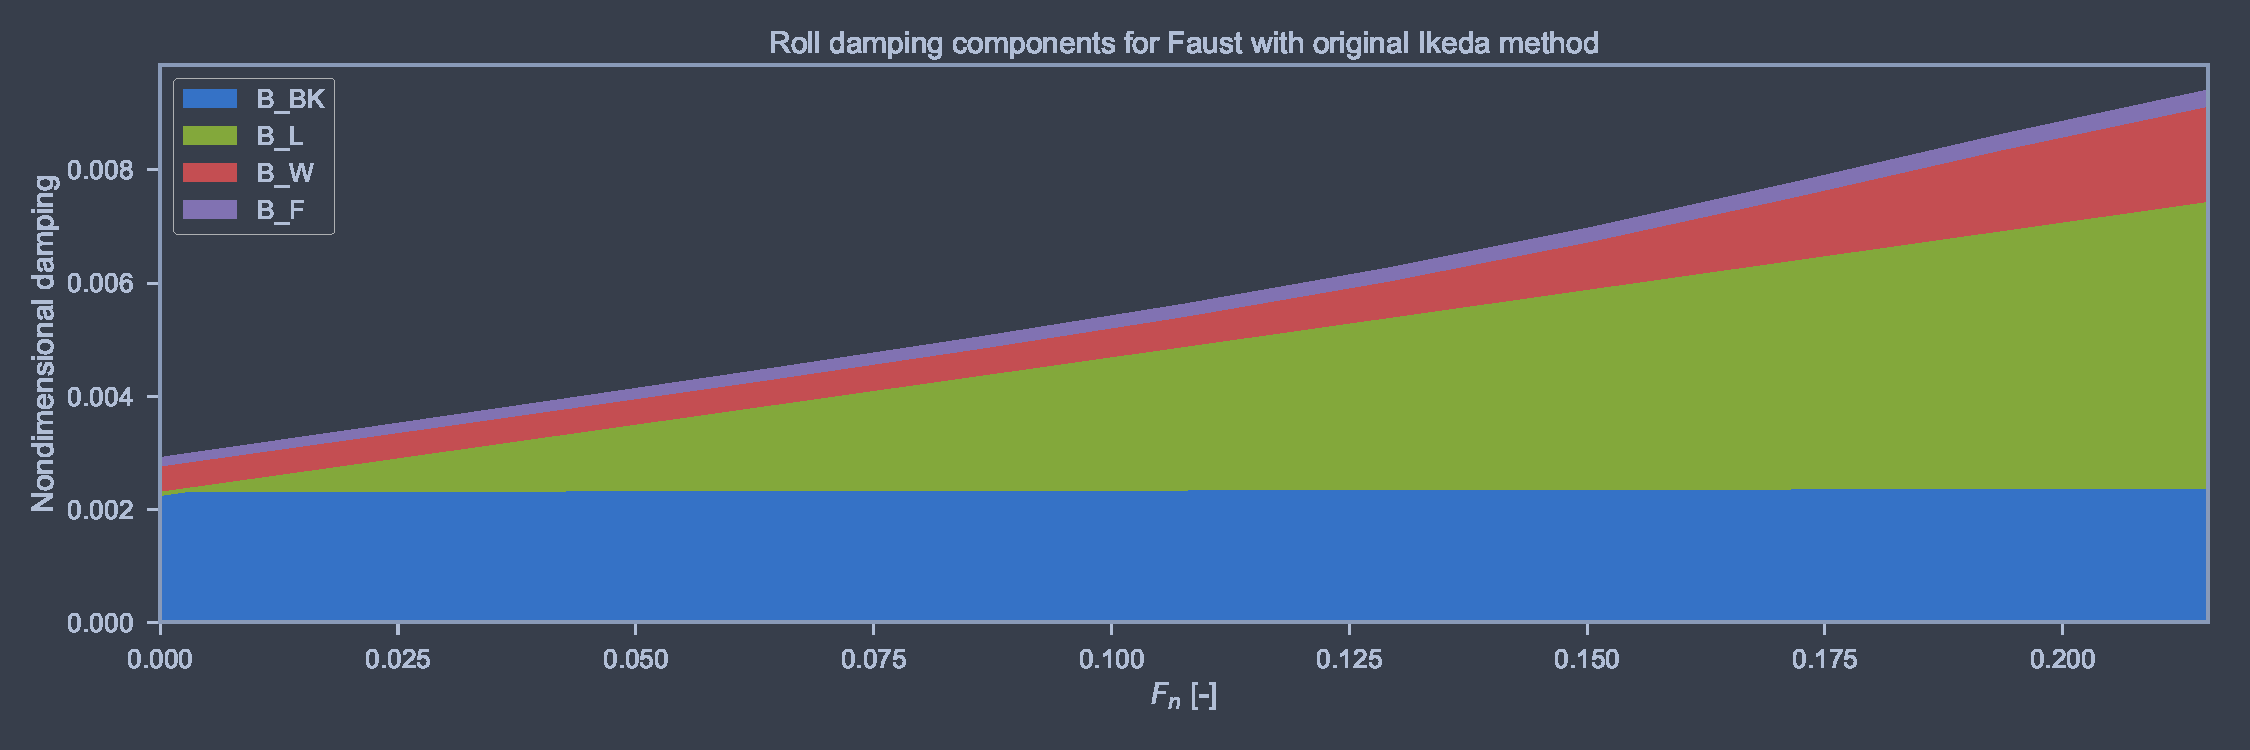
\includegraphics[]{figures/ikeda_faust.pdf}
    \caption{Roll damping components calculated with Ikeda method for PCTC Faust}
    \label{fig:ikeda_faust}
\end{figure}



Ikedas original method require strip method calculations. This is not an attractive option for the present study since that would require calculations with exact hull geometries to be carried out for all of the ships in the study. There exist however a \emph{Simplified Ikeda method} \cite{kawahara_simple_2011} that is instead used in this study \emph{Simplified Ikeda method} predicts the roll damping components at zero speed.

A study of the has been conducted which shows the roll damping components for various speeds. Calculations with *Ikeda original method* and the *Simplified method* have been carried for two ships (*S175* and *Faust*). The two methods show reasonable agreement for zero speed.

In order to introduce a speed dependancy to the *Simplified method* the following is conducted:
* Add Lift damping $B_L$.
* Add speed dependence of wave damping $\frac{B_W}{B_{W0}}$
* Remove $B_E$ at ($F_n>0.15$) ?